% Bagian: sets-functions-relations
% Bab: relations
% Subbagian: trees

\documentclass[../../../include/open-logic-section]{subfiles}

\begin{document}

\olfileid[id]{sfr}{rel}{tre}
\olsection{Pohon}

Satu jenis khusus urutan parsial yang berperan penting dalam semua bagian
logika adalah \emph{pohon}. Pohon hingga muncul dalam bagian-bagian dasar
logika: misalnya, !!{formula}s dapat dipahami melalui penguraiannya menjadi
pohon sintaksis, sedangkan !!{derivation}s dalam banyak sistem
!!{derivation} juga berbentuk pohon hingga.
%
Pohon tak hingga sudah muncul dalam pembuktian teorema kelengkapan untuk
logika proposisional dan logika orde pertama, serta digunakan di seluruh
logika matematika.

Konsep pohon dalam teori himpunan berkaitan erat dengan gagasan pohon dalam
teori graf. Berikut gambar sebuah pohon (hingga):

\begin{center}
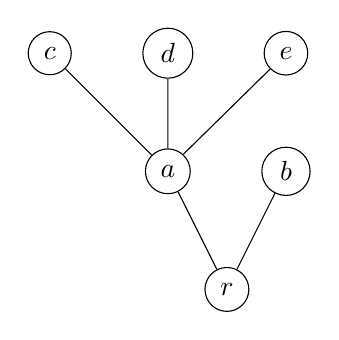
\begin{tikzpicture}[nodes={draw, circle}, -]
\node{$r$} [grow'=up]
    child { node {$a$}
        child { node {$c$} }
        child { node {$d$} }
        child { node {$e$} }
    }
    child { node {$b$} };
\end{tikzpicture}
\end{center}

Simpul paling bawah~$r$ adalah akar. Setiap simpul selain $r$ mempunyai tepat
satu simpul induk yang berada tepat di bawahnya. Kita dapat memandang relasi
antara simpul~$x$ dan simpul~$y$, ketika $y$ dapat dicapai dari~$x$ dengan
mengikuti sisi ke atas, sebagai relasi bahwa $x$ merupakan \emph{leluhur}
dari~$y$.

Relasi leluhur dalam suatu pohon merupakan urutan parsial ketat. Hal ini
memotivasi definisi berdasarkan teori himpunan. Untuk menyatakannya, kita
memerlukan dua konsep. Suatu \emph{elemen terkecil} dalam himpunan~$A$ yang
diurutkan secara parsial oleh~$\le$ adalah !!a{element} $x \in A$ sedemikian
sehingga, untuk semua $y \in A$, berlaku $x \le y$. Suatu himpunan
\emph{terurut baik}
oleh~$\le$ jika setiap himpunan bagiannya yang tak kosong mempunyai elemen
terkecil.

\begin{defn}[Pohon]
Suatu \emph{pohon} adalah pasangan $T = \tuple{A, \le}$ sedemikian sehingga
$A$ merupakan himpunan dan $\le$ merupakan urutan parsial pada~$A$ dengan
elemen terkecil tunggal $r \in A$ (disebut \emph{akar}), serta untuk semua
$x \in A$, himpunan $\Setabs{y}{y \le x}$ terurut baik oleh~$\le$.
\end{defn}

\begin{defn}[Penerus]
Andaikan $T = \tuple{A, \le}$ merupakan pohon. Jika $x,y \in A$, $x < y$,
dan tidak ada $z \in A$ sedemikian sehingga $x < z < y$, maka kita mengatakan
bahwa $y$ merupakan \emph{penerus} dari~$x$.
\end{defn}

Penerus-penerus dari $x \in A$ juga disebut \emph{anak-anaknya}. Jika
$y$ merupakan penerus dari~$x$, kita menyebut $x$ sebagai \emph{pendahulu}
atau \emph{induk} dari~$y$.

\begin{prop}
Jika $\tuple{A,\le}$ merupakan pohon, maka setiap $x \in A$ selain akar
mempunyai paling banyak satu pendahulu.
\end{prop}

\begin{proof}
  Andaikan $y_1 < x$, $y_2 < x$, dan $y_1 \neq y_2$. Maka
  $\{y_1, y_2\} \subseteq \Setabs{z}{z<x}$. Karena $\Setabs{z}{z<x}$ terurut
  baik oleh~$\le$, himpunan bagiannya $\{y_1, y_2\}$ mempunyai elemen
  terkecil, yang jelas harus berupa $y_1$ atau~$y_2$. Jadi, $y_1 \le y_2$
  atau $y_2 \le y_1$. Kita mengasumsikan $y_1 \neq y_2$, sehingga sebenarnya
  $y_1 < y_2$ atau $y_2 < y_1$. Karena kita juga mengasumsikan $y_1 < x$ dan
  $y_2 < x$, maka $y_1 < y_2 < x$ atau $y_2 < y_1 < x$. Jadi, $y_1$ dan $y_2$
  tidak mungkin keduanya merupakan pendahulu dari~$x$.
\end{proof}

\begin{defn}
Suatu pohon $T = \tuple{A, \le}$ disebut \emph{tak hingga} jika $A$ merupakan
himpunan tak hingga dan disebut \emph{hingga} jika tidak demikian. Jika $T$
sedemikian sehingga setiap $x \in A$ hanya mempunyai berhingga banyak
penerus, kita mengatakan bahwa $T$ \emph{bercabang hingga}.
\end{defn}

\begin{defn}[Cabang]
Untuk suatu pohon $T = \tuple{A, \le}$, \emph{cabang} dari~$T$ adalah rantai
maksimal dalam~$T$, yakni himpunan $B \subseteq A$ sedemikian sehingga untuk
setiap $x, y \in B$ berlaku $x \le y$ atau $y \le x$, dan untuk setiap
$z \in A \setminus B$ terdapat $u \in B$ sedemikian sehingga $z \le u$ maupun
$u \le z$ tidak berlaku.
%
Kita menggunakan $[T]$ untuk menyatakan himpunan semua cabang dari $T$.
\end{defn}

\begin{ex}
Contoh klasik pohon bercabang hingga adalah \emph{pohon biner tak hingga}
yang terdiri atas barisan hingga dari $0$ dan~$1$, kadang-kadang dinotasikan
dengan $\{0,1\}^*$ atau~$\Bin^*$, dan diurutkan oleh relasi perluasan
$\sqsubseteq$ (misalnya, $101 \sqsubseteq 101101$). Karena setiap untai biner
selalu dapat diperluas dengan menambahkan $0$ atau $1$ di ujungnya, pohon ini
memuat tak hingga banyak elemen: setiap elemen~$s$ mempunyai tepat dua
penerus, $s0$ dan~$s1$. Akarnya adalah barisan kosong $\emptyseq$.
\end{ex}

\begin{ex}
Secara sedikit lebih umum, himpunan barisan hingga bilangan asli~$\Nat^*$
dengan relasi perluasan~$\sqsubseteq$ juga merupakan pohon. Jelas bahwa pohon
ini tidak bercabang hingga: setiap $s \in \Nat^*$ mempunyai tak hingga banyak
penerus~$sn$, satu untuk setiap $n \in \Nat$. Setiap himpunan tak kosong
$A \subseteq \Nat^*$ yang tertutup terhadap~$\sqsubseteq$ merupakan
\emph{subpohon} dari~$\Nat^*$.
(Artinya, $A$ sedemikian sehingga jika $s \in A$ dan $s' \sqsubseteq s$, maka
$s' \in A$.) Semua pohon hingga dapat direpresentasikan sebagai subpohon
hingga dari~$\Nat^*$.
\end{ex}

\begin{prop}[Lema K\H{o}nig]
Jika $T = \tuple{A,\le}$ merupakan pohon tak hingga yang bercabang hingga,
maka $T$ mempunyai cabang tak hingga.
\end{prop}

Suatu kasus khusus lema K\H{o}nig yang digunakan secara luas dalam teori
komputabilitas, dan dikenal sebagai \emph{lema lemah K\H{o}nig}, berbunyi
sebagai berikut: setiap subpohon tak hingga dari $\{0,1\}^*$ mempunyai cabang
tak hingga.

\end{document}
